%%%%%%%%%%%%%%%%%%%%%%%%%%%%%%%%%%%%%%%%%%%%%%%%%%%%%%%%%%%%%%%%%%%%%%%%%%%%%%
%
\section{Method}
\label{sec:method}
%    3.1  Overall framework p5
%    3.2  Dictionary and Sparse space p6-p8
%    3.3  Dimensionality reduction to grayscale p8-p11
%
%%%%%%%%%%%%%%%%%%%%%%%%%%%%%%%%%%%%%%%%%%%%%%%%%%%%%%%%%%%%%%%%%%%%%%%%%%%%%%

\begin{figure}[t]
\begin{center}
\begin{tabular}{ccc}		
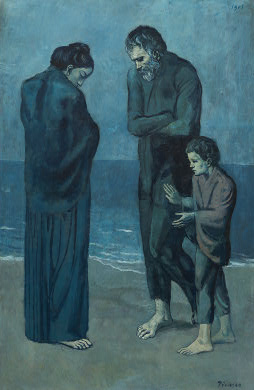
\includegraphics[width=0.3\linewidth]{fig/Poor-nga.jpg} &
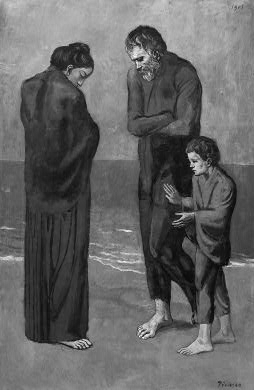
\includegraphics[width=0.3\linewidth]{fig/Poor-nga-sparse_dr.png} & 
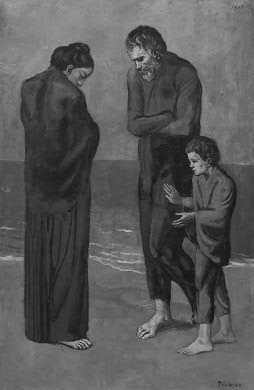
\includegraphics[width=0.3\linewidth]{fig/Poor-nga-rgb2gray.png} \\
(a) The Tragedy & (b) Our result & (c) rgb2gray
\end{tabular} 	
\end{center}
\caption{Emotional impression depicted in various blues is lost after decolorization.}
\label{fig:difficulty}
\end{figure}

As we have discussed in the previous section, 
most of the existing techniques to convert a color image 
into grayscale do attempt to address preserving not only the luminance 
but also the chromatic information. 
However, their formulation often investigates the related features 
either in the original color space or 
in yet another color space of the same dimension. 
In our method, we instead transform the 3-D color space 
into a new feature space of higher-dimensions. 
We achieve this effect by learning an image-dependent dictionary $D$
to account for the important features such as color and saliency distributions.
To go from the original color space to this new space, 
denoted as $F^{|D|} \subseteq \mathbb{R}^{|D|}$, 
without significantly increasing the computational complexity,
we consider a sparse linear model \cite{Seeger08:BIO} over $D$,
and more significantly, 
we show that the underlying relations among the luminance and chromatic features
can be better revealed in $F^{|D|}$. 
Hence, designing a transformation to carry out color conversion 
by preserving the relations there would generally lead to a more effective scheme.

%
\subsection{Overall framework}
\label{sec:framework}
%

The main challenge of decolorization is the loss of visually
meaningful chromatic information, which in certain cases is extremely hard
to maintain after converting to a grayscale image. 
Take, for example, the famous painting ``The Tragedy'' by Pablo Picasso 
shown in Figure~\ref{fig:difficulty}. Without relying parameter hand-tuning,
most of the state-of-the-art techniques or softwares for decolorization 
would not be able to capture the emotional impression depicting by the various blues.
One main reason for the difficulty is that visually meaningful contents
inspired by chromatic stimuli cannot be appropriately represented in a 3-D color space.
And it causes most of the related techniques to fail. 
Nevertheless, as we will describe later, chromatic information of less subtlety
can be more satisfactorily retained in a systematic framework over $F^{|D|}$.

\ignore{
\begin{figure}[t]
\begin{center}
\begin{tabular}{c}
\psfrag{RGB}{{\sssmall RGB}}
\psfrag{linear transformation}{{\sssmall linear projection $P$}}
\psfrag{inner product}{{\sssmall inner product}}
\psfrag{preserving}{{\sssmall preserving}}
\psfrag{grayscale}{{\sssmall grayscale}}
\psfrag{feature space}{{\sssmall feature space}}
\psfrag{F}{{\sssmall $F^{|D|}$}}		
\psfrag{Dictionary}{{\sssmall dictionary $D$}}	
\includegraphics[height=2.0in]{fig/overview.eps}
\end{tabular} 	
\end{center}
\caption{The linear projection $P$ is to preserve the feature relations in $F^{|D|}$.}
\label{fig:overview}
\end{figure}
}

Motivated by the recent success in adopting the sparse linear model
to tackle various vision applications, we propose a decolorization method 
that the formulation is established based on the assumption: 
{\em The luminance and the chromatic features of an image 
are better described in $F^{|D|}$ than in the original color space.}
This is in general true since, contrary to a universal color space, 
$F^{|D|}$ is specifically constructed for each image. 
A sparse linear model can be expressed by

\begin{equation}
\mathbf{x} = D \mathbf{c} + \epsilon
\label{eqn:sparse}
\end{equation}

\noindent where $\epsilon$ is a Gaussian noise, 
and the coefficients in $\mathbf{c}$ are assumed to be i.i.d. 
drawn from a Laplace distribution. 
To perform decolorization, we begin by adaptively learning a dictionary 
from a given color image. 
The resulting dictionary would reasonably encode the {\em principal} luminance 
and chromatic information. 
We further consider the {\em lasso} model \cite{Tibshirani94} of sparse coding
to conveniently locate the mapping from the color space to the feature space 
induced by the dictionary. 
Finally, a closed-form solution to perform dimensionality reduction 
from the new space to the grayscale space is then applied to complete the color conversion.
In Figure~\ref{fig:overview}, we illustrate the whole procedure of our approach.

%
\subsection{Dictionary learning}
\label{sec:dict}
%

Given a color image $I = \{\mathbf{x}_i = (r_i, g_i, b_i)^T\}_{i=1}^n$ of $n$ pixels, 
we apply the image segmentation algorithm by Felzenszwalb and 
Huttenlocher~\cite{Felzenszwalb:2004:EGI} to derive a collection of superpixels, 
and calculate the mean color vector $ \mathbf{m}_j = (r_j, g_j, b_j)^T$ of each segment $j$.
To emphasize those that are visually significant, 
we also compute a saliency map using the method presented in \cite{Goferman10}.
The sum of the saliency values for pixels in segment $j$ is denoted as $s_j$. 
We further assume that $\{ \mathbf{m}_j\}$ is arranged as a sorted list 
in a descending order of $s_j$.

To construct a dictionary $D$ for decolorizing $I$, we need a pool $\Omega$ 
of possible atoms, which are collected by sequentially adding $\mathbf{m}_j$ to the pool,
if it is sufficiently {\em dissimilar} to those already in $\Omega$, \ie,

\begin{equation}
\mathrm{dist}(\mathbf{m}_j, \Omega) = \min\limits_{\mathbf{m}_k \in \Omega} \mathrm{dist}(\mathbf{m}_j, \mathbf{m}_k) < \delta
\label{eqn:delta}
\end{equation}

\noindent where $\delta$ is a parameter, and set to $0.3$ in all our experiments.
Apparently, $\Omega$ is a still a sorted list, 
and indeed a refined set of $\{ \mathbf{m}_j\}$. 
Our criterion for an ideal $D$ is that it should include atoms with large $s_j$, 
and meanwhile each of them should play a significant role in the sparse coding. 
More precisely, suppose we have chosen a subset of atoms from $\Omega$ to yield $D$.
It is thus preferable that the atoms are from the front end of $\Omega$. 
To check whether $D$ is a proper dictionary for sparse coding with respect to $I$,
we solve the following lasso problems:

\begin{equation}
\min\limits_{\mathbf{c}_i} \frac{1}{\alpha^2} \| \mathbf{x}_i - D\mathbf{c}_i \|^2_2 + \frac{1}{\beta} \|\mathbf{c}_i\|_1
\label{eqn:lasso}
\end{equation}

\noindent for all $\mathbf{x}_i \in I$, 
where the two parameters in (\ref{eqn:lasso}) are related by $\alpha^2/\beta = 0.05$
as suggested in \cite{YangYH10}. 
The scatter matrix of $I$ under the mapping $\mathbf{x}_i \mapsto \mathbf{c}_i$ is given by

\begin{equation}
M = \sum\limits_i (\mathbf{c}_i-\bar{\mathbf{c}})(\mathbf{c}_i-\bar{\mathbf{c}})^T
\label{eqn:scatter}
\end{equation}

\noindent where $\bar{\mathbf{c}}$ is the mean of $\{\mathbf{c}_i\}$. 
When $M$ is not full-rank, it implies that there exist {\em non-informative} atoms in $D$,
and they are not used (or rarely used) in performing sparse coding for $I$.
For a color image of a large size, solving (\ref{eqn:lasso}) for all pixels 
is time-consuming. 
In that case, a downsample version of $I$ will instead be considered. 
We describe a practical implementation for learning $D$ in Algorithm~\ref{Alg:dictionary}
that can avoid a naive and time-consuming way of sequentially adding the atoms to construct
$D$ until the condition of full rank is violated.

\begin{algorithm}[tH]
\SetKwInOut{Input}{Input} %
\SetKwInOut{Output}{Output} %
\DontPrintSemicolon %
\SetAlgoLined %
\Input{An image $I=\{\mathbf{x}_i\}$ of tatal saliency value $s$,
a sorted list $P=\{\mathbf{m}_j\}$ with its corresponding $\{s_j\}$,
and a parameter $ r \in (0.5,1]$.}%
\Output{$D$.} %
\BlankLine %
1. $r \leftarrow \min\{r, {\sum_j s_j}/s\}$.\; %
2. Initialize $D$ by selecting the least $k$ atoms from $P$ such that $\sum_{j=1}^k s_j/s \ge r$.\; %
3. $J \leftarrow \mathrm{downsample}(I)$. \; %
4. Solve the lasso problem (\ref{eqn:lasso}) for all $\mathbf{x}_i \in J$. \;%
5. Compute the scatter matrix $M$ as in (\ref{eqn:scatter}).\;%
6. \If{$M$ is not full-rank}{
       Remove the last $k-\mathrm{rank}(M)$ atoms from $D$.\;%
       $k \leftarrow |D|$.\;%
       Repeat steps 4, 5, and 6.\;%
    }{return $D$}
\caption{Learning $D$ for decolorization. \label{Alg:dictionary}}
\end{algorithm}

% advantage higher space without redundancy cf. main-theme vector
% justifications why full-rank , zeros of _ci , unnecessary,


It is insightful to discuss the properties of $D$ in more detail. 
First, observe that the resulting dictionary is established by including 
as many atoms as possible, 
providing it would not break the full-rank condition on the scatter matrix of the sparse coefficient vectors. By enforcing this constraint, 
our method does not introduce extra and unnecessary feature dimensions 
in transforming the color space to the $F^{|D|}$. 
As we will see in the next section, 
this nice property of $D$ is also useful in finding the exact form of 
the linear projection to the grayscale space. 
Second, the atoms of $D$ are {\em representative} as they are considered 
in a descending order of the sum over the saliency values of their respective pixels 
so that each atom corresponds to the mean color vector of 
either a large or a salient segment. 
We also require them to significantly account for the saliency distribution of $I$. 
(See Algorithm~\ref{Alg:dictionary}).

%
\subsection{Grayscale conversion}
\label{sec:grayscale}
%

We are now ready to discuss how to carry out the linear projection 
to convert a color image into grayscale. 
Since we are to preserve the feature relations in $F^{|D|}$ after performing 
linear projection, we consider solving the following optimization problem:

\begin{equation}
\min_{P} \sum_i \sum_j (\mathbf{c}_i - \mathbf{c}_j)^T(P\mathbf{x}_i - P\mathbf{x}_j)
\label{eqn:optimization}
\end{equation}

\noindent where $P$ is a 1-D linear projection (\ie, a $1\times 3$ matrix) 
form the input color space to the grayscale space. 
In solving (\ref{eqn:optimization}), we first need to solve the lasso problem 
defined in (\ref{eqn:lasso}) for all pixels in $I$,
which would be impractical for images of large sizes. 
However, owing to the lasso model (\ref{eqn:lasso}) in linking $\mathbf{x}_i \in I$ 
and its sparse code $\mathbf{c}_i$, a closed-form solution of (\ref{eqn:optimization}) 
derived by Gkioulekas and Zickler \cite{Gkioulekas:2011:DRU} can be directly applied. 
It follows that

\begin{equation}
P = L R = \mathrm{diag}(f(\lambda)) \mathbf{V}^T R
\label{eqn:projection}
\end{equation}
\noindent where
\begin{equation}
f(\lambda) = \left(\frac{4\beta^4\lambda}{\alpha^4+4\beta^2\alpha^2\lambda+4\beta^4\lambda^2}\right)^{1/2}
\label{eqn:f}
\end{equation}
\noindent
and $\lambda$ is the largest eigenvalue of the matrix $D^TD$, 
$\mathbf{V}$ is the corresponding eigenvector, 
$\alpha$ and $\beta$ are the parameters in (\ref{eqn:lasso}), 
and $R$ is a $3 \times 3$ rotation matrix to be decided. 
Recall that the dictionary $D$ is derived by adding the mean vector $\mathbf{m}_j$ 
according to a descending order of saliency values, 
while respecting the full-rank constraint. 
The criterion can help not only avoid introducing unnecessary feature dimensions 
but also measure the {\em goodness} of a rotation matrix. 
To that end, we consider solving

\begin{equation}
\max_{R} \sum\limits_{j=1}^{|D|} \sum\limits_{k=1}^{|D|} s_j (P\mathbf{m}_j - P\mathbf{m}_k)^2 = \sum\limits_{j=1}^{|D|} \sum\limits_{k=1}^{|D|} s_j (LR\mathbf{m}_j - LR\mathbf{m}_k)^2\,.
\label{eqn:rotation}
\end{equation}

The optimization problem (\ref{eqn:rotation}) is to seek for an optimal rotation matrix $R$
such that the saliency features can be preserved after the dimensionality reduction. 
Solving (\ref{eqn:rotation}) is nontrival, and the quality of a local-minimal 
``solution'' heavily depends on the initial guess of $R$. 
We instead ``solve'' (\ref{eqn:rotation}) by uniformly sampling a large number of 
3-D rotation matrices, and adopt the one with the maximal objective value for our use. 
In all our experiments, we generate 100,000 such matrices, and the technique 
empirically achieves better performance than optimizing (\ref{eqn:rotation}) 
using the identity matrix as a starting point.
